\documentclass{article}
\usepackage{algorithm}% http://ctan.org/pkg/algorithm
\usepackage{algpseudocode}% http://ctan.org/pkg/algorithmicx
\usepackage{subcaption}
\usepackage{graphicx}

%%%%%% More sensible page sizes %%%%%%%
\usepackage[a4paper]{geometry}

%%%%%% MATH MACROS %%%%%%%
\usepackage{amssymb}
\usepackage{amsthm}
\usepackage{mathtools} 

%%%%%%%% [ocimathesis] MACROS %%%%%%%
\usepackage{hyperref}
\usepackage{enumitem}

%%%%%%  OTHER MACROS %%%%%%%%%%%
\usepackage{todonotes}

%%%%%%%%% CRYPTOCODE MACROS %%%%%%%%%

\let\etoolboxforlistloop\forlistloop % save the good meaning of \forlistloop
\usepackage[n, advantage, operators, sets, adversary, landau, logic,
events, complexity, asymptotics, operators, keys, probability,
notions, ff, primitives, mm]{cryptocode}
\let\forlistloop\etoolboxforlistloop % restore the good meaning of \forlistloop

%%%%%%%%%%% NEW ENVIRONMENTS %%%%%%%%%
\newtheorem{theorem}{Theorem}[section]
\newtheorem{definition}[theorem]{Definition}

%%%%%%%%%% NEW COMMANDS %%%%%%%%%%%%
\newcommand{\esk}{\textsf{esk}}
\newcommand{\sigm}[2]{\sig_{sk_{#1}}(#2)}
\newcommand{\gensigm}[1]{\sigm{}{#1}}
\newcommand{\botsig}{\gensigm{\bot}}
\newcommand{\abotsig}[1]{\sigm{#1}{\bot}}
\newcommand{\myconcat}{ \;||\; }

\newcommand{\newconsgen}[1]{\prf(#1 \myconcat \botsig, \mathrm{tag} )}
\newcommand{\newconspi}{\newconsgen{\pi(x)}}

% We're doing alphabetical by default
\author{
  Liliya Akhmetzyanova\\
  \texttt{lah@cryptopro.ru}
  \and
  Cas Cremers\\
  \texttt{cremers@cispa.saarland}
  \and
  Luke Garratt\\
  \texttt{lgarratt@cisco.com}
  \and
  Stanislav V. Smyshlyaev\\
  \texttt{smyshsv@gmail.com}
}
\title{Security Analysis for Randomness Improvements for Security
Protocols}

\date{v1.1 -- March 25th, 2019}
\begin{document}
  \maketitle

%\pagenumbering{arabic}

\begin{abstract}
Many cryptographic mechanisms depend on the availability of secure
	random numbers. In practice, the sources of random numbers can
	be unreliable for many reasons. There exist ways to improve the
	reliability of randomness, but these often do not work well with
	practical constraints.
	One proposal to reduce the impact of untrusted randomness is the
	proposal by Cremers et al.~\cite{randomnessirtf}, which aims to
	be effective in existing deployments.

	In this document, we provide a security analysis of the
	construction in~\cite{randomnessirtf} (Revision 3) and elaborate
	on design choices and practical interpretations.
\end{abstract}

\section{Introduction}
All key exchange protocols (e.g., SSL/TLS, SSH, IKE, etc.) depend on the generation of secure random numbers. At the core of all of these protocols is a Diffie--Hellman key exchange of the following basic form: Alice chooses random number $x$, computes $g^x$ and sends it to Bob. Bob similarly chooses random number $y$, computes $g^y$ and sends it to Alice. Of course, each particular protocol has other essential details such as certificates, signatures, key derivation, comparing of transcripts and so on, but at the heart of all these protocols is the shared secret $g^{xy}$. Therefore, it is essential that $x$ and $y$ are generated as securely as possible. 

In many operating systems, raw entropy comes in the form of events such as mouse movements or keystrokes. As large amounts of raw entropy is difficult to accumulate, Alice and Bob do not generate truly random numbers $x$ and $y$ for their key exchanges. Instead, they use the primitive of a cryptographically secure pseudorandom number generator (CSPRNG), which takes as input a seed, continually harvests more raw entropy and  produces arbitrary many pseudorandom numbers as required. Since CSPRNGs are used to provide the essential secret $g^{xy}$, they clearly need to be as secure as possible. 

However, the current problem we face is that all CSPRNGs depend on raw entropy in some form or another. Therefore, if the underlying randomness is not good, the secret $g^{xy}$ is not secure. Real-world examples of poor random number generation include:

\begin{itemize}
\item The Debian OpenSSL random number generator vulnerability \cite{DebianRNGflaw, DebianRNGflawTLSDHE};

\item Predictable random numbers in Android's Java OpenSSL \cite{MarvinGoogle2013} leading to theft of bitcoins;

\item The Dual EC random number generator backdoor \cite{DualECstandardisedbackdoor};

\item Random number generator on hardware that degrades over time;

\item Servers that are deployed in settings where good randomness generation cannot be guaranteed;

\item Internet of Things (IoT) devices with good (factory) keys but no good randomness generation after deployment.
\end{itemize}

We propose a solution to this problem. Our solution is inspired by the
so-called ``NAXOS trick'' for key exchange protocols. In contrast to the
NAXOS trick, our design is more generic and applies outside of the AKE
domain, and we follow a much more conservative approach that enables the
re-use of existing infrastructure and improved graceful degradation if
it turns out the hash function's output may reveal partial information
from the output.

From the academic literature on authenticated key exchange protocols, the NAXOS protocol \cite{LaMacchiaeCK2007} does not just compute pseudorandom numbers $x$ and $y$ from raw entropy and send $g^{x}$ and $g^{y}$, but instead sends $g^{H(x, \sk_{\hat A})}$ and $g^{H(y, \sk_{\hat B})}$ where $H$ is a random oracle, and $\sk_{A}$ and $\sk_{B}$ are the long-term secret keys of Alice and Bob respectively. Intuitively we can see that securely in this case should now depend on the pairs ($x$, $\sk_{\hat A})$ and ($y$, $\sk_{\hat B})$ being secure, as opposed to just $x$ and $y$ being secure. What is more, a protocol that uses $g^{H(x, \sk_{\hat A})}$ can behave in exactly the same way as one that uses $g^x$. The only essential difference is that $H(x, \sk_{\hat A})$ is a safer secret than $x$.

In this note, we take an alternative approach for real-world protocols.
In particular, often the long-term term $\sk$ is in trusted hardware so
it is impossible to have direct access to it to compute $H(x, \sk)$.
For many HSM deployments, this prevents the application of the NAXOS
trick.
Moreover, a choice needs to be made as to what function implements the
random oracle $H$. We will also need to know precisely what security
guarantees our construction provides.  We will answer these questions
and provide proofs that are construction meet precisely definition
security guarantees under standard cryptographic assumptions. We will
show that our construction improves the generation of pseudorandom
numbers and provides concrete security guarantees for a generic class of
protocols including SSL/TLS, SSH, IKE, etc. at negligible cost to efficiency. 

\subsection*{Our wrapper construction}

We propose a ``wrapper'' function around existing
pseudorandom number generators, in contexts that have access to a
party's signing algorithm. Let $y$ be the output of the pseudorandom
number generator which length is equal to the KDF output length. As in the main document~\cite{randomnessirtf}, we define the wrapper to be:

$$
\prf(\texttt{KDF}( \texttt{H}(\sig (\sk, \texttt{tag}_1)),y), \texttt{tag}_2, n),
$$
where $\texttt{tag}_1$ and $\texttt{tag}_2$ are public and are chosen
from some fixed sets $\mathcal{T}_1$ and $\mathcal{T}_2$ correspondingly
and where \texttt{PRF} and \texttt{KDF} and instantiated with
HKDF-expand and HKDF-extract respectively.
We encourage the reader to see the main document~\cite{randomnessirtf} for full details.

\subsection*{Overview}
In Section \ref{CSPRNG} we recall the standard properties of a CSPRNG. In Section \ref{sec:def} we define the security properties we will need for our primitives in our wrapper construction. In Section \ref{sec:model} we define our security model for our wrapper construction. In Section \ref{proof} we give a security theorem and formal game hopping security proof it fulfils the security properties we claim. We make additional notes on the real-world security of our wrapper construction in Section \ref{sec:notes}.
In Appendix~\ref{experiments} we provide the results of experiments aimed to investigate the effect of the wrapper implementing on performance.

\section{Background on CSPRNGs} \label{CSPRNG}
Forward secure cryptographically secure pseudorandom number generators (CSPRNG) are already used as primitives in TLS and other protocols. Let Rand be a forward secure CSPRNG. By this we mean Rand satisfies the following two properties:

\subsubsection*{Property 1. Indistinguishable from random (CSPRNG)}

A family of deterministic polynomial time computable functions $Rand_{\lambda}
\colon \{0, 1\}^{\lambda} \rightarrow \{0, 1 \}^{p(\lambda)}$ for some polynomial
$p$ is a  CSPRNG, if it stretches the length of its input ($p(\lambda) > \lambda$ for any $\lambda$) and if its output is computationally indistinguishable from true randomness, i.e. for any probabilistic polynomial time algorithm $A$, which outputs 1 or 0 as a distinguisher,

$$ \left \vert \Pr_{x\gets\{0,1\}^\lambda}[A(Rand(x))=1] - \Pr_{r\gets\{0,1\}^{p(\lambda)}}[A(r)=1] \right \vert < \mu(k) $$

\noindent for some negligible function $\mu$.

All this is saying is that, no efficient algorithm (with knowledge of how Rand works) can distinguish the output of Rand from randomness, when the initial seed is unknown and uniformly random. Note that achieving this property is non-trivial: many pseudorandom number generators may achieve output that looks statistically random, but does not satisfy this property. For instance, the function that hashes the initial seed to produce $x$. Then hashes $x$. Then hashes again, and so on, could produce statistically random output, but an efficient adversary that knows how this algorithm works can clearly distinguish this from purely random behaviour after seeing the first two blocks of output (the second being the hash of the first).

Andrew Yao showed that this definition is equivalent to the next-bit test (below).

\subsubsection*{Property 2. Resistance to state compromise extensions (forward secure)}
Another property we want is for the CSPRNG to be forward secure. A forward-secure CSPRNG with block length $t(\lambda)$ is a $Rand_{\lambda} \colon \{0,1\}^\lambda \to \{0,1\}^\lambda \times \{0,1\}^{t(\lambda)}$, where the input string $s_i$ with length $\lambda$ is the current state at period $i$, and the output $s_{i+1}$, $y_i$ consists of the next state $s_{i+1}$ and the pseudorandom output block $y_i$ of period $i$, such that it withstands state compromise extensions in the following sense. If the initial state $s_1$ is chosen uniformly at random from $\{0,1\}^\lambda$, then for any $i$, the sequence $(y_1, y_2,\dots, y_i,s_{i+1})$ must be computationally indistinguishable from $(r_1,r_2,\dots,r_i,s_{i+1})$, in which the $r_i$ are chosen uniformly at random from $\{0,1\}^{t(\lambda)}$.

\subsubsection*{The next-bit test (equivalent definition of CSPRNG)}
By satisfying the next-bit test, we mean that given the first $\lambda$ bits of outputs from $Rand$ sequence, there is no polynomial-time algorithm that can predict the $(\lambda+1)$th bit with probability of success better than 50\% (without knowing the seed). Andrew Yao proved in 1982 that a generator passing the next-bit test will pass all other polynomial-time statistical tests for randomness.

Let $P$ be a polynomial, and $S=\{S_\lambda\}$ be a collection of sets such that $S_\lambda$ contains $(\lambda)$-bit long sequences. Moreover, let $\mu_\lambda$ be the probability distribution of the strings in $S_\lambda$.

Let $\mathcal{M}$ be a probabilistic Turing machine, working in polynomial time. Let $p_{\lambda,i}^{\mathcal{M}}$ be the probability that $\mathcal{M}$ predicts the $(i+1)$st bit correctly, i.e.

$$p_{\lambda,i}^{\mathcal{M}}=\Pr[M(s_1\ldots s_i)=s_{i+1}\ | \ s\in S_\lambda\text{ with probability }\mu_\lambda(s)]$$

We say that collection $S = \{ S_\lambda \}$ passes the next-bit test if for all polynomial $Q$, for all but finitely many $\lambda$, for all $0 < i < \lambda$: 

$$
p_{\lambda,i}^{\mathcal M}<\frac{1}{2}+\frac{1}{Q(\lambda)}
$$

\section{Security definitions} \label{sec:def}

Here we will precisely define the security properties we need of our primitives for our construction to be proven secure in our security model.

\subsection{Key derivation function} \label{KDFdef}
A key derivation function is an algorithm $\texttt{KDF}$ that implements a deterministic function $k=\texttt{KDF}(x, y)$, taking as input some bit strings $x$ and $y$, and returning a key $k \in \{0,1\}^h$. We require $\texttt{KDF}$ to fulfill two following security properties. 

\textbf{KDF security.} Intuitively, this property means computational indistinguishability of the $\texttt{KDF}(x,\cdot)$ function for $x$ chosen uniformly at random from an ideal random function $\rho(\cdot)$. Namely, it is the standard PRF security property. Let $\epsilon_{\texttt{KDF}}$ denote the probability that any probabilistic polynomial time adversary is able to distinguish between these distributions.

\textbf{Uniformness preserving.} We require the $\texttt{KDF}$ algorithm to fulfill the uniformness preserving of the output for $y \sample \{0,1\}^h$ chosen uniformly at random and $x$ chosen arbitrarily. 
We define a security game between an adversary $A$ and a challenger as follows.

\begin{enumerate}
	\item The adversary makes a query $x$. The challenger uniformly randomly samples a secret value $y \sample \{0,1\}^h$. The challenger computes $k_0 \coloneqq \texttt{KDF}(x,y)$ and samples $k_1 \sample \{0,1\}^h$ uniformly randomly. The challenger then flips a coin $b \sample \{0, 1\}$ and responds with $k_b$.
	
	\item The adversary then outputs a guess $b'$ for $b$ and wins the game if $b = b'$ and loses otherwise.
\end{enumerate}

Let $\epsilon_{\texttt{UP}}$ denote the probability that any probabilistic polynomial time adversary is able to win the considered above game. In other words, for any probabilistic polynomial time algorithm $A$	
$$
\left \vert \Pr(b = b') - \frac{1}{2} \right \vert \le \epsilon_{\texttt{UP}}.
$$

The  $\texttt{KDF}$ algorithm is said to be $\texttt{UP}$-secure if $\epsilon_{\texttt{UP}}$ is negligible in security parameter~$n$.

\paragraph{HKDF-extract.}

In our concrete construction, we instantiate \texttt{KDF} with HKDF-extract that is literally the HMAC function.  There are two ways to use  HKDF-extract: with direct order of arguments ($\texttt{KDF}(x,y) := \text{HKDF-extract}(x,y)$) and with reverse one ($\texttt{KDF}(x,y) := \text{HKDF-extract}(y,x)$). 

Let start with reverse order of arguments where the hashed signature is used as a message input for HMAC. In the case when CSPRNG is broken and controlled by adversary, the required PRF property for $\texttt{KDF}$ is crucial. Therefore, we expect that the HMAC function with swapped inputs should remain prf-secure. Note that such a security property has not been investigated and if we do not model HMAC as a random oracle there is a necessity to analyze this property carefully.

Consider the direct order of arguments. For this case the first KDF property is believed due to the prf-security of the HMAC construction (see{~\cite{BellareCK1996} for more detail). Moreover, for the wrapper the length of the HMAC key $x = \texttt{H}(\sig (\sk, \texttt{tag}_1))$ is equal to the hash output length that satisfies recommendations.    
	
	Consider the uniformness preserving property for the HKDF-extract function basing on a hash function \texttt{H} with good combinatorial properties. Precisely, for this function the following balance property holds:	
$$\Pr_{y \sample \{0,1\}^h}[ \texttt{H} (x\|y) = k ] = \frac{1}{2^h},\ \forall\ k \in \{0,1\}^h,\ x \in \{0,1\}^*.$$

It easy to see that for HKDF-extract, that is purely $\texttt{HMAC} (x,y) = \texttt{H}(x_{opad}\|\texttt{H}(x_{ipad}\|y))$, the same property holds. Thus, the uniformness preserving property is fairly supposed to hold. The same can be shown for the reverse order of arguments.


\subsection{Variable-length output pseudorandom function} \label{PRFdef}

%\todo[inline]{In order to prove the security with multiple tag1 I need to use a multi-user security definition for PRF. I believe that the reduction to the standard one-key security can be easily done using the hybrid argument. CC: Looks good to me.}

A variable-length output pseudorandom function is an algorithm $\prf$ that implements a deterministic function $z=\prf(k, c, n)$, taking as input a key $k \in \{0,1\}^h$, some bit string $c$, an integer $n$, and returning a string $z \in \{0, 1 \}^{n}$. We assume that the maximum permitted size $n$ is polynomial. %For brevity we will omit the parameter $n$ assuming that the $\prf$ algorithm returns the values of the maximum permitted size.

We define a security game (for multi-user setting) between an adversary $A$ and a challenger as follows.

\begin{enumerate}
	\item The challenger uniformly randomly samples $t$ (polinomial) secret keys $k_1,\ldots,k_t \in \{0,1\}^h$ independently from each other.
	
	\item The adversary is allowed to query the challenger with adaptively chosen values $(i,c,n)$, $i \in [1,\ldots,t]$. The challenger replies with $\prf(k_i, c,n)$.
	
	\item Eventually the adversary queries a special symbol $T$ to indicate the so-called test query with value $(i,c,n)$ where $(i,c,\cdot)$ was not queried before. At this point, the challenger computes $z_0 \coloneqq \prf(k_i, c,n)$ and samples $z_1$ uniformly randomly. The challenger then flips a coin $b \sample \{0, 1\}$ and responds with $z_b$.
	
	\item The adversary is allowed to keep making queries. Note that after the test query the adversary is not allowed to query $(i,c,\cdot)$.
	
	\item The adversary then outputs a guess $b'$ for $b$ and wins the game if $b = b'$ and loses otherwise.
\end{enumerate}

Let $\epsilon_{\texttt{mu-}\prf}$ denote the probability that any probabilistic polynomial time adversary is able to win the considered above game. In other words, for any probabilistic polynomial time algorithm~$A$	

$$
\left \vert \Pr(b = b') - \frac{1}{2} \right \vert \le \epsilon_{\texttt{mu-}\prf}.
$$

The  $\prf$ algorithm is said to be $\texttt{mu-}\prf$-secure if $\epsilon_{\texttt{mu-}\prf}$ is negligible in security parameter~$\lambda$.



%\begin{enumerate}
%\item Initially the adversary chooses on which of the argument the adversary wants to attack and send the decision to the challenger makes the initial query containing the string $\texttt{x}$ or $\texttt{y}$. The challenger samples either $y$ or $x$ respectively uniformly randomly, computes and returns the value $\texttt{KDF}(y, x)$.

%\item Next, the challenger computes $z_0 \coloneqq \texttt{KDF}(y, x)$ and samples $z_1$ uniformly randomly. It flips a coin $b \sample \{0, 1 \}$ and gives $z_b$ to the adversary.

%\item The adversary outputs a guess $b'$ for $b$. The adversary wins if $b' = b$ and loses otherwise.
%\end{enumerate}

%The advantage of any probabilistic polynomial time adversary winning the above security game should be negligible in the security parameter. In other words,

%$$
%\left \vert \Pr(b = b') - \frac{1}{2} \right \vert \le \epsilon_{\texttt{KDF}}
%$$

\subsection{Hash function and signature scheme}
A signature scheme is a triple $(\kgen, \sig, \verify)$. $\kgen$ is a probabilistic algorithm which takes as input the security parameter $1^\alpha$ and outputs a public signature verification key $\pk$ and secret signing key $\sk$. $\sig$ is a signing algorithm which generates a signature $\sigma$ for message $m$ using secret key $\sk$. In the current paper we consider only deterministic $\sig$ algorithms. $\verify$ is a deterministic signature verification algorithm which, given input $(\pk, \sigma, m)$, outputs $1$ if $\sigma$ is a valid signature of $m$ under key $\pk$, and $0$ otherwise. It is required that for every $k$, every $(\sk, \pk)$ output by $\kgen (1^\alpha)$, and every message $m$, it holds that

$$\verify (m , \sig ({\sk, m})) = 1$$

In our construction, we will not want to use the long-term key $\sk$ directly. We will instead use the hash of a signature of $\texttt{tag}_1$, signed with $\sk$. For our security proof, we require the combined hash function and signature scheme to fulfil the following  security property.

Consider the following game between a challenger and a polynomial time adversary $A$:

\begin{enumerate}
\item The challenger generates a public/private key pair $(\pk, \sk)$ using $\kgen$ and gives the adversary the public key $\pk$. %Then the adversary sends the $\mathrm{\texttt{tag}_1}$ value to the challenger.

\item The adversary is allowed to query adaptively chosen messages $m$ to the challenger. The
challenger responds to each query with $\sigma=
\sig{(\sk, m})$. 

\item When the adversary decides to, it outputs a so-called test query $m^*$ that was not queried before. At this point, the challenger flips an unbiased coin $b \sample \{0, 1\}$. If heads, it returns with $ \texttt{H}(\sig (\sk, m^*))$. If tails, it responds with a uniformly random string of the same length.

\item The adversary is allowed to keep asking for signatures with messages $m \neq m^*$, but eventually it must output a guess $b'$ for the coin flip $b$, at which point the game ends. The adversary wins if it guesses the coin flip correctly and loses otherwise.
\end{enumerate}

Let $\epsilon_{\sig, \texttt{H}}$ denote the probability that any probabilistic polynomial time adversary is able to win the considered above game. In other words, for any probabilistic polynomial time algorithm~$A$		
$$\left \vert \Pr(b = b') -\frac{1}{2} \right \vert \le \epsilon_{\sig, \texttt{H}}.$$

The  ($\sig$, $\texttt{H}$) composition is said to be $\sig, \texttt{H}$-secure if $\epsilon_{\sig, \texttt{H}}$ is negligible in security parameter~$\alpha$.

This security property can be instantiated with routine cryptographic assumptions such as a hash function behaving as a random oracle and an existentially unforgeable signature scheme.

\section{Security model} \label{sec:model}
Here we define the security property we expect from our wrapper in terms of a game between a challenger and an adversary.

We run a game between the challenger and the adversary as follows. At the beginning of the game the challenger uniformly randomly chooses a secret key $\sk$ and returns a public key $\pk$ to the adversary. Receiving the public key the adversary chooses a set $T \subseteq \mathcal{T}_1$ consisting of $l$ pairwise different values $t_1,\ldots,t_l$ and sends it to the challenger.  We assume that the size $l$ of the set $T$ are polynomial. 

% \todo[inline]{There will be some problems with the proof if we allow the
% adversary to choose tag1 values adaptively. Namely, in Case1, Game2. The
% HSig adversary does not know what tag1 will be test and cannot trivially provide the correct responses for non-test output queries with same tag1 that were made before test query. If you will solve this problem we can extend the model. } 
% 
% \todo[inline]{Luke: it seems the best we can do is guess it in advance as it belongs to some small set, or restrict it as per the rules of the game. Currently it is the former.}

The adversary is allowed to make the following queries to the challenger.


\begin{itemize}
	
	\item The adversary can make \texttt{output} queries of two types:
	\begin{itemize}
		\item $\texttt{tag}_1, \texttt{tag}_2, n$ (in this case the challenger chooses the $y \sample \{0,1\}^h$ value uniformly randomly by itself);
		\item $\texttt{tag}_1, \texttt{tag}_2,y,n$ (in this case the $y \in \{0,1\}^h$ value is chosen by the adversary).
	\end{itemize}
	
	Note that the adversary is allowed to make queries where $\texttt{tag}_1 \in T$. 
	
	The challenger produces $$
	\prf(\texttt{KDF}(\texttt{H}(\sig (\sk,\texttt{tag}_1)), y), \texttt{tag}_2,n)
	$$
	and returns this value as a response to the corresponding \texttt{output} query.
	
	The challenger indexes queries and locally saves the corresponding inputs to the wrapper for each query, i.e. the challenger saves records of the form $(i,\texttt{tag}_1^i,\texttt{tag}_2^i,y_i)$.  We assume that $i \le M$ for some M that is also polynomial.
	
	\item The adversary can make \texttt{sign} queries for signatures with $\sk$ of messages $m$. The challenger produces and returns the value $\sig (\sk, m)$.
	
	\item The adversary can make \texttt{corrupt} query for $\sk$ at any time. The challenger must respond with $\sk$ to this query.
	
	\item The adversary is also allowed to make \texttt{reveal} queries for the $y_i$ value used in the $i$th \texttt{output} query at any time (the adversary makes the query with the index of the target \texttt{output} query). The challenger must respond with the $y_i$ value used in generating the response to the $i$th \texttt{output} query.
	
	\item We say that the $i$th \texttt{output} query is "fresh" if one of the values $y_i$ and $\mathrm{\texttt{signature}}$ stay secret. That is, if one of the following conditions is satisfied:
	\begin{itemize}
		\item the adversary has not made the \texttt{corrupt} query or the \texttt{sign} query for $m = \texttt{tag}_1^i$. 
		\item this query fixes only $\texttt{tag}_1, \texttt{tag}_2 , n$ and the adversary has not made the \texttt{reveal} query for  $y_i$.
	\end{itemize}
	
	We also say that an \texttt{output} query is "non-trivial" if one of the following conditions is satisfied
	
	\begin{itemize}
		\item this query is of the first type $\texttt{tag}_1, \texttt{tag}_2, y, n$ where query with $\texttt{tag}_1, \texttt{tag}_2, y$ has not been made before. 
		
		\item this query is of the second type $\texttt{tag}_1, \texttt{tag}_2, n$.  
	\end{itemize}
	
	
	At some point in time, the adversary must make a so-called test \texttt{output} query. This is the same as a normal non-trivial \texttt{output} query except the challenger flips an unbiased coin and either responds with the genuine output using the wrapper, or a uniformly randomly chosen string of the same length. 
	
	\item The adversary is allowed to query for the $y$ used in the test if it wants to, as well as to continue making other queries. The adversary may also query for the $\sk$ value or for the signature of $\texttt{tag}_1$ if it has not already done so. However, the test output query must remain fresh at all times during the game.
	
	\item At some point in time after the test query, the adversary must output a single bit as a guess. The adversary wins the game if it is able to guess the coin flip with non-negligible advantage over $\frac{1}{2}$.
\end{itemize}

\section{Proof of security} \label{proof}

\begin{theorem}
If $\prf$, $\texttt{KDF}$, $\sig$ and $\texttt{H}$ satisfy the security definitions above, then any probabilistic polynomial time adversary has only negligible advantage in winning the security game.	
\end{theorem}

\begin{proof}
	Let Game 0 denote the original security game as defined in our security model definition. Let $S_j$ denote the event of the adversary winning Game $j$. Our goal in this proof is to bound $\Pr(S_0)$ to show that it is only at most negligibly above $\frac{1}{2}$. Although the security argument is very intuitive (``the adversary must surely need both $y$ and $\sk$ to guess the secret'') we will formally prove it in a game hopping proof.

At some point in time, the adversary must issue a \texttt{test} query. Let $\texttt{tag}_1^i, \texttt{tag}_2^i, y_i$ denote the values used by the challenger for this query. We prove this theorem in a case partition on whether the adversary has revealed $\sig(\sk,\texttt{tag}_1^i)$ or $y_i$. (If the adversary has queried for neither, then it is clearly in an even worse position to win the game.) 

\noindent We now proceed with our case partition.

\subsubsection*{Case 1: The adversary has revealed $y_i$ or has chosen $y_i$ by itself.} In this case, the adversary is not allowed to query for $\sk$ or for the signature of $\texttt{tag}_1^i$, otherwise the test output query would not be fresh.

\noindent \textbf{Game 1.} Let Game 1 be identical to Game 0 except the challenger guesses in advance an integer $j \in [1, \dots, l]$ and aborts (and the adversary loses) unless $\texttt{tag}_1^i = t_j$.  This is a large failure event game hop and it is easy to see that

$$
\Pr(S_0) \le l \Pr(S_1)
$$


\noindent \textbf{Game 2.} Define Game 2 to be identical to Game 1 except $\texttt{H}(\sig(\sk, \texttt{tag}_1^i))$ is replaced with a value $x_i$ sampled uniformly at random for each  \texttt{output} query with $\texttt{tag}_1 = \texttt{tag}_1^i$. Here we claim that
$$\Pr(S_1) \le  \Pr(S_2) + \epsilon_{\texttt{H}, \sig}$$

In particular, no probabilistic polynomial time distinguisher algorithm can distinguish between Game 1 and Game 2, since this would imply a way to beat the hash-signature game with better than $\epsilon_{\texttt{H}, \sig}$ advantage. Precisely, an adversary in the hash-signature game could beat it with better than $\epsilon_{\texttt{H}, \sig}$ advantage as follows. 

It acts as a challenger in the hybrid game and inserts the value of $\pk$ from the hash-signature game. As an adversary in the hash-signature game, it inserts the known $\texttt{tag}_1$ value from the previous game and asks a test query straight away, receiving either $ \texttt{H}(\sig (\sk, \texttt{tag}_1^i))$ or a uniformly randomly chosen value $x_i$ as per the rules of the hash-signature game. It inserts this value as the value for $ \texttt{H}(\sig (\sk, \texttt{tag}_1^i))$ in the hybrid game. Because of Game 1, the adversary knows where to make this swap in the game. The \texttt{output} queries with $\texttt{tag}_1 \neq t_j$ are processed by the adversary using queries for signature to its challenger.  The adversary can now simulate \texttt{output} and test queries as normal using this value. The adversary does not have to worry about simulating a \texttt{corrupt} query because we are in case 1. Finally, it can simulate signature queries by merely forwarding them along into the hash-signature game. This perfectly simulates the hybrid game: it is literally Game 1 if the test returns $ \texttt{H}(\sig (\sk, \texttt{tag}_1^i))$, and it is literally Game 2 if it returns a uniformly randomly chosen value $x_i$. The adversary follows the coin flip choice in the simulated hybrid game as its guess for the hash-signature game. By assumption of the hardness of the hash-signature game, all adversaries can only win with at most advantage $\epsilon_{\texttt{H}, \sig}$. Therefore, the difference in advantages of adversaries across Game 1 and Game 2 can also only be separated by at most $\epsilon_{\texttt{H}, \sig}$. Thus the claim above is proven.

\noindent \textbf{Game 3.} Define Game 3 to be identical to Game 2 except 
$\texttt{KDF}(x_i,\cdot)$ is replaced with an ideal random function $\rho(\cdot)$ for \texttt{output} query with $\texttt{tag}_1 =t_j$. Here we claim that

$$
\Pr(S_2) \le \Pr(S_3) + \epsilon_{\texttt{KDF}}
$$

Here we present the simulation argument for the KDF game. Because of Game 1, the adversary knows where to make this swap in the game precisely for \texttt{output} queries with  $\texttt{tag}_1 =t_j$. The KDF adversary makes queries $y$ to compute $\texttt{KDF}(x_i,y)$ for required $y$ for the key $x_i$ chosen by the challenger uniformly at random.  If the adversary has made the $(\texttt{tag}_1,\texttt{tag}_2,n)$ query (without $y$), then the KDF adversary chooses $y$ value uniformly randomly by itself and locally saves it. Note that it can answer the reveal query in this case. All other queries are simulated in the normal way. This perfectly simulates the hybrid game: it is literally Game 2 if the KDF challenger provides outputs of the $\texttt{KDF}$ function, and it is literally Game 3 if the challenger provides outputs of the ideal random function $\rho$. The adversary follows the coin flip choice in the simulated hybrid game as its guess for the KDF game. By assumption of the hardness of the KDF game, all adversaries can only win with at most advantage $\epsilon_{\texttt{KDF}}$. Therefore, the difference in advantages of adversaries across Game 2 and Game 3 can also only be separated by at most $\epsilon_{\texttt{KDF}}$. Thus the claim above is proven.

\noindent \textbf{Game 4.} Define Game 4 to be identical to Game 3 except the response to the test \texttt{output} query is replaced with a value chosen uniformly randomly.

Here we claim that
$$
\Pr(S_3) \le \Pr(S_4) + \epsilon_{\texttt{mu-}\prf}
$$

Here we present the simulation argument for the multi-user PRF game with at most $M$ keys.  Because of Game 1, the PRF adversary knows what \texttt{output} queries should be processed with the usage of its challenger. The \texttt{output} queries with $\texttt{tag}_1 =t_j$ and different $y$ are processed with the different keys by asking the mu-PRF challenger with the suitable indexes in queries. Since the test query should be non-trivial, $y_i$ or $\texttt{tag}_2^i$ should be new (we neglect the probability that for the \texttt{output} query of the type $(\texttt{tag}_1,\texttt{tag}_2,n)$ the $y_i$ value chosen by the challenger itself collides with the previous values). Therefore, the mu-PRF adversary can use its test query to swap the $\prf(\rho(y_i), \texttt{tag}^i_2, n)$ with the value obtained as a response on the test query in the mu-PRF game. All other queries are simulated in the normal way. This perfectly simulates the hybrid game. Therefore, the difference in advantages of adversaries across Game 2 and Game 3 can also only be separated by at most $\epsilon_{\texttt{PRF}}$. Thus the claim above is proven.

It is clearly impossible for the adversary to have any advantage in guessing the secret bit in Game 4 (in either case, the wrapper generates a uniformly randomly chosen string). As such, $\Pr(S_4) = \frac{1}{2}$. Thus in this case $\Pr(S_0) \le \frac{1}{2} + l( \epsilon_{(\texttt{H}, \sig)} + \epsilon_{\texttt{KDF}} + \epsilon_{\texttt{mu-}\prf})$ which is negligibly close to~$\frac{1}{2}$.

\subsubsection*{Case 2: The adversary has revealed $\sk$ or $\sig(\sk, \texttt{tag}_1^i)$.}

In this case, the adversary is not allowed to reveal $y_i$ or to choose $y_i$ by itself, otherwise the test output query would not be fresh. Thus, $y_i \in \{0,1\}^h$ is chosen uniformly randomly by the challenger and is used only for the test \texttt{output} query.  

%%% CC: Commented out for now since we don't need to.
%\todo[inline]{Luke: Did we need an intermediate game hop to guess the test $\texttt{tag}_1$ here? If so, it is in both cases so we should put it before the case distinction. And we mean to replace only the KDF output with the test $\texttt{tag}_1$ right?}

\noindent \textbf{Game 1.} This game is identical to Game 0 except $\texttt{KDF}(\texttt{H}(\sig (\sk, \texttt{tag}^i_1)), y_i)$ for test \texttt{output} query is replaced with a value $k$ sampled uniformly at random. 

We claim that 		
$$
\Pr(S_0) \le \Pr(S_1) + \epsilon_{\texttt{UP}}
$$

In the simulation the UP adversary for $\texttt{KDF}$ chooses private key $\sk$ by itself and simulates all queries except for the test \texttt{output} query in the normal way. To simulate the test \texttt{output} query $(\texttt{tag}^i_1, \texttt{tag}^i_2, n)$ the UP adversary makes a query with  $\texttt{H}(\sig (\sk, \texttt{tag}^i_1))$ to its UP challenger. The challenger chooses $y_i \sample \{0,1\}^h$ and returns a value $k_b$. Then the UP adversary computes and returns the value $\prf(k_b,\texttt{tag}^i_2, n)$.  This perfectly simulates the hybrid game. Therefore, the difference in advantages of adversaries across Game 0 and Game 1 can also only be separated by at most $\epsilon_{\texttt{UP}}$. Thus the claim above is proven.

\noindent \textbf{Game 2.} Define Game 2 to be identical to Game 1 except the response to the test \texttt{output} query is replaced with a value chosen uniformly randomly.

Here we claim that
$$
\Pr(S_1) \le \Pr(S_2) + \epsilon_{\texttt{mu-}\prf}
$$

The simulation is the same as for Game 4 from the other case but here is enough to make one test query for one key in the multi-user PRF game since the key $k$ is used once for the test \texttt{output} query only.

It is clearly impossible for the adversary to have any advantage in guessing the secret bit in Game 2 (in either case, the wrapper generates a uniformly randomly chosen string). As such, $\Pr(S_2) = \frac{1}{2}$. Thus in this case $\Pr(S_0) \le \frac{1}{2} + \epsilon_{\texttt{UP}} + \epsilon_{\texttt{mu-}\prf}$ which is negligibly close to~$\frac{1}{2}$.
\end{proof}

\section{Real-world considerations} \label{sec:notes}

\subsection{Design choices}
Which of our primitives are chosen for real-world reasons and which are useful for the security proof? Our security proof could be done even more easily by using directly $\sk$ instead of $\sig(\sk, \texttt{tag}_1)$. However, in the real-world it is preferable to keep the secret key in an HSM and only perform certain operations on it such as making signatures. There is no guarantee that the signature is uniformly distributed as a key, so this is why we hash it and chose $\texttt{H}(\sig(\sk, \texttt{tag}_1))$ over $\sk$. Consequently, this also is why one of the security assumptions of our theorem is the difficulty of the ``hash-signature game''. The practical interpretation we are asking of the challenger is merely that the signature is a secret the adversary cannot guess, just like $\sk$.

The $\texttt{KDF}$ and $\texttt{PRF}$ constructions are useful in practice because they are easily available, and they help in the security proof. In fact, the security assumptions we require of them for the proof are very minimal indeed. 
In our concrete construction, we recommend to implement them as HKDF-extract and HKDF-expand respectively. As mentioned in Section \ref{KDFdef}, in the case of reverse order of arguments one should be aware of our assumption regarding the prf-security of the HMAC scheme with swapped inputs.

The tags are assumed to be known in our security model. In practice they may not be, which only adds an extra layer of protection in practice.

In no case can our wrapper construction be worse than not having it all. In the usual case, we merely depend on $y_i$ being secret. With our wrapper construction, we essentially use $\texttt{KDF}(y_i \concat x)$ for an $x$ which may or may not be known. One may wonder how the signature is generated: probabilistic or deterministic? Could this be a chicken and egg problem, noting that in many signature schemes, if random numbers are bad and the signature is leaked, then the secret key is leaked? Thus, if random numbers are bad in the first place, the signature will be bad, and thus the construction will not be of any use. This is why we require that the signature scheme is deterministic.

\subsection{Practical interpretations}
The security model and consequent proof refers heavily to the concept of ``freshness'', which intuitively encodes the adversary not winning the game trivially by making the obvious reveal queries. The practical interpretation of our security theorem is as follows. If the adversary learns only one of the signature or the usual randomness generated on one particular instance, then under the security assumptions on our primitives, the wrapper construction should output randomness that is indistinguishable from a random string.

Our security model also explicitly assumes that $\sig (\sk, \texttt{tag}_1)$ never appears externally elsewhere in
the protocol so that the adversary has no hope of seeing it and using it. Otherwise, security degrades to the normal case of generating pseudorandom numbers. Of course, in practice actually
forcing $\sig (\sk, \texttt{tag}_1)$ to appear may still be difficult.  Note furthermore that these
signatures are agent-specific, which improves containment. Thus, leaking
or forging $\sig (\sk_{\hat A}, \texttt{tag}_1)$ for a specific agent $\hat A$ only affects $\hat A$, and
has no consequences for other agents.  The fact that in reality $\texttt{tag}_1$ is separate for each application and $\texttt{tag}_2$ changes also helps to prevent repeated random numbers when there is a poor entropy source. 

\vspace{10pt}

\noindent \textbf{Acknowledgments}

\vspace{10pt}

The authors would like to thank Christopher Wood for providing implementation experiments.  

\bibliographystyle{plain}
\bibliography{masterbib}

\begin{appendix}
	
\section{Randomness Wrapper Experiments}\label{experiments}
	We implemented the randomness wrapper in C using the BoringSSL library.
We implemented the Extract and Expand routines using HKDF-Extract and HKDF-Expand, as described
in \cite{hkdfrfc}. To understand the relative
overhead of the wrapper primitives, we also implemented a CMAC-based KDF, with similar Extract and Expand routines desribed in \cite{ckdfirtf}. With our implementation, we then ran the following wrapper and baseline
experimental algorithms detailed in Algorithm \ref{alg:wrapper-experiment} and \ref{alg:baseline-experiment},
respectively, with configuration inputs $sk$, $\mathtt{tag}_1$, and $\mathtt{tag}_2$, and block
size $B$, loop count $n$, and hash size $L$. The wrapper experimental algorithm computes the signature
\emph{once} and reuses it for all subsequent extractions. By varying the number of loops, we can measure
the rate at which continued use amortizes the signature computation cost. $\mathsf{Now}$ is a function
that returns the current time in nanoseconds.

\begin{algorithm}
	\caption{Wrapper Experimental Algorithm}\label{alg:wrapper-experiment}
	\begin{algorithmic}[1]
		\State $t_s \gets \mathsf{Now()}$
		\State $s \gets \mathsf{Hash}(\mathsf{Sign}(\mathsf{sk}, \mathtt{tag}_1))$
		\For{$n$ loops}
		\State $y \gets \mathsf{G}(L)$
		\State $k \gets \mathsf{Extract}(k, s)$
		\State $r \gets \mathsf{Expand}(k, \mathtt{tag}_2, B)$
		\EndFor
		\State $t_e \gets \mathsf{Now()}$
		\State \textbf{return} $t_e - t_s$
	\end{algorithmic}
\end{algorithm}

\begin{algorithm}
	\caption{Baseline Experimental Algorithm}\label{alg:baseline-experiment}
	\begin{algorithmic}[1]
		\State $t_s \gets \mathsf{Now()}$
		\For{$n$ loops}
		\State $r \gets \mathsf{G}(B)$
		\EndFor
		\State $t_e \gets \mathsf{Now()}$
		\State \textbf{return} $t_e - t_s$
	\end{algorithmic}
\end{algorithm}

Figures \ref{fig:exp-a}, \ref{fig:exp-b}, \ref{fig:exp-c}, and \ref{fig:exp-d} show results
from our experiments, when run on a Macbook Pro laptop with a $3.3$ GHz Intel Core i7 CPU and
$16$GB or RAM. The delta between the wrapper and baseline experimental algorithm is shown
as a function of the loop count in each plot for both HKDF (with SHA256) and CKDF (with a $16$B
key). Each plot uses a fixed extraction length $B$, including $32$, $128$, $256$, and $1024$ bytes.
We chose these values as they reflect common extraction lengths for protocols such as TLS, e.g.,
where a random Curve25519 key is derived from $32$ random bytes.

Results indicate that caching the signature output is critical for performance. For nearly
all block sizes, the cost levels out towards an asymptote at approximately $1,000$ loops.
At this point, both KDF variants perform nearly equally well (with the exception of $B = 1024$,
where CKDF performs favorably to HKDF), and cost approximately three orders of magnitude
more than the baseline algorithm ($\mathsf{G}$), i.e., from nanoseconds to microsecondss.
However, the relative cost is minor with respect to cryptographic operations in protocols
such as TLS.

\begin{figure}[H]
	\begin{subfigure}{.5\textwidth}
		\centering
		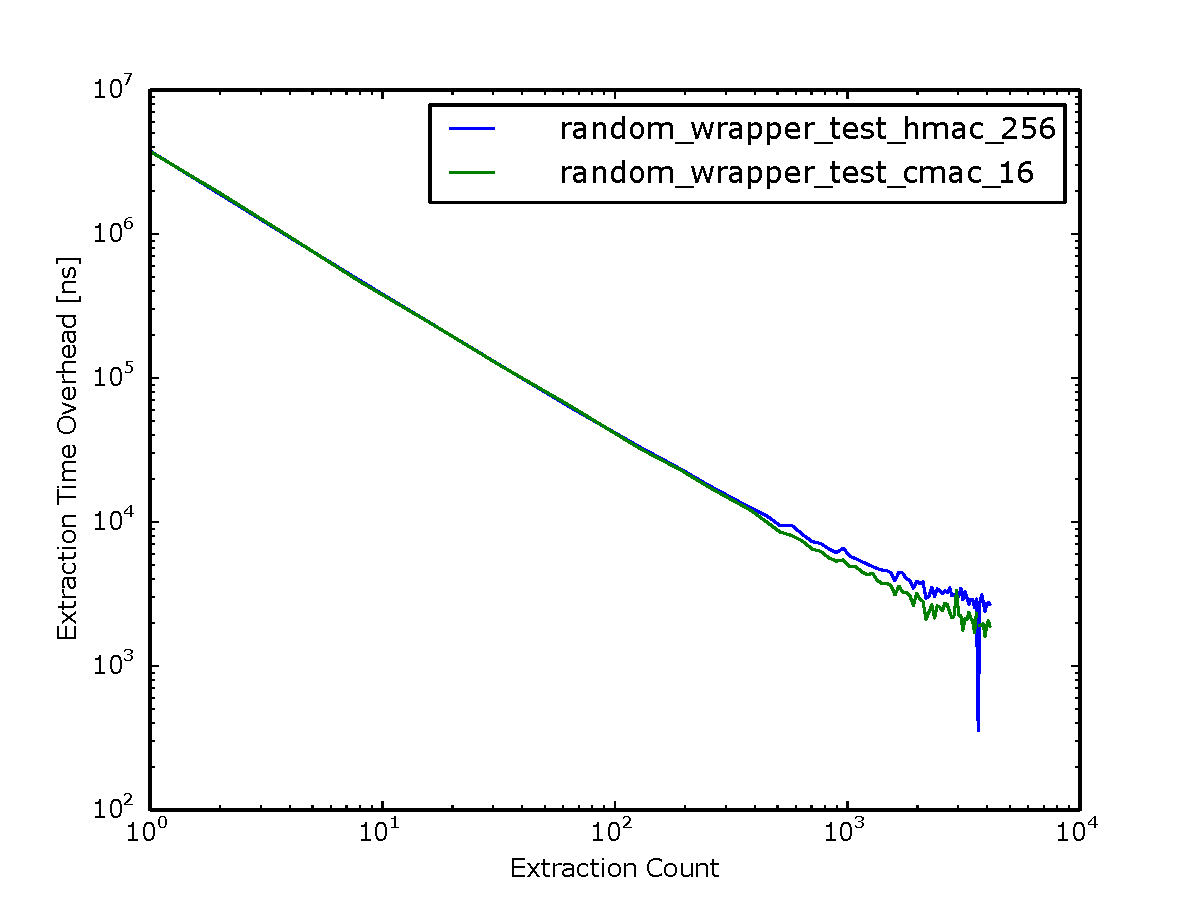
\includegraphics[width=\linewidth]{cost_32.pdf}
		\caption{$B = 32$}
		\label{fig:exp-a}
	\end{subfigure}
	\hfill
	\begin{subfigure}{.5\textwidth}
		\centering
		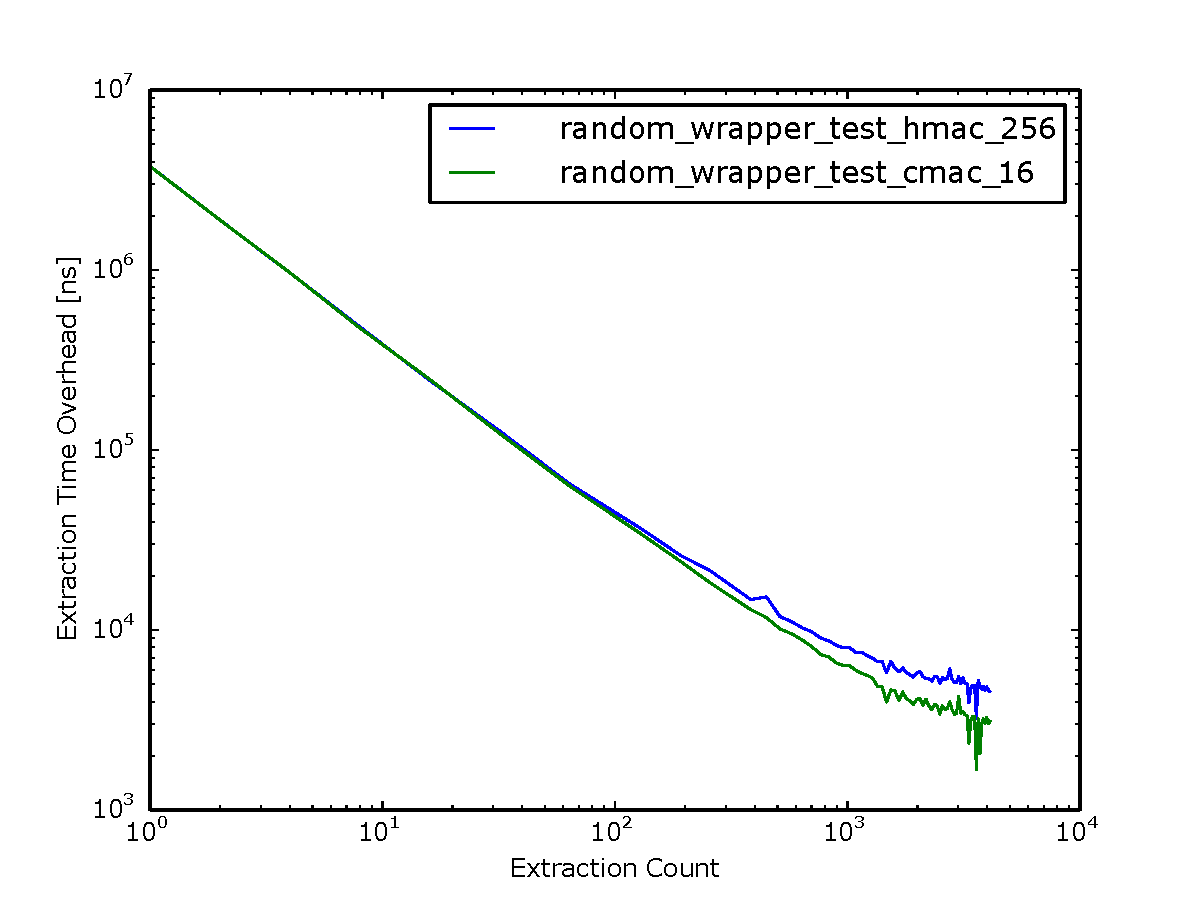
\includegraphics[width=\linewidth]{cost_128.pdf}
		\caption{$B = 128$}
		\label{fig:exp-b}
	\end{subfigure}
	\hfill
	\begin{subfigure}{.5\textwidth}
		\centering
		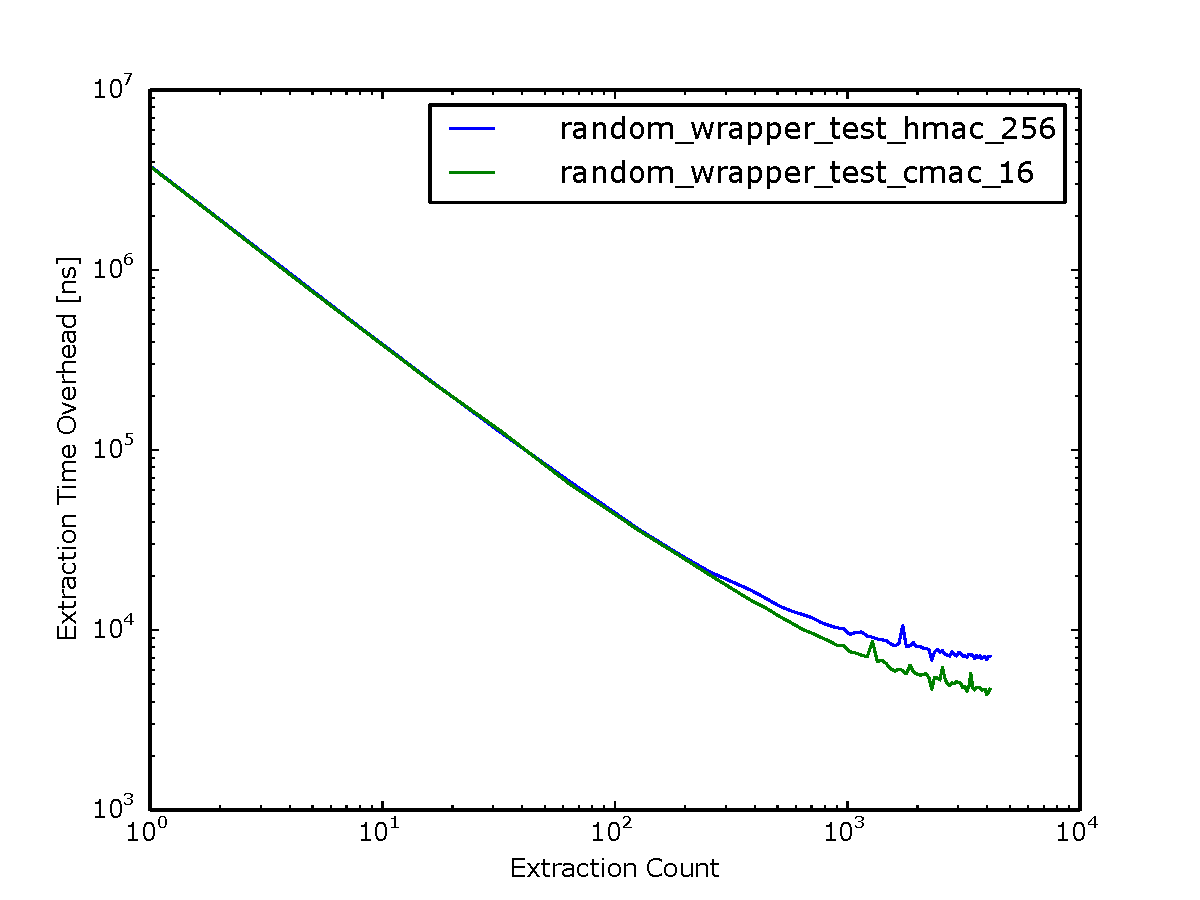
\includegraphics[width=\linewidth]{cost_256.pdf}
		\caption{$B = 256$}
		\label{fig:exp-c}
	\end{subfigure}
	\begin{subfigure}{.5\textwidth}
		\centering
		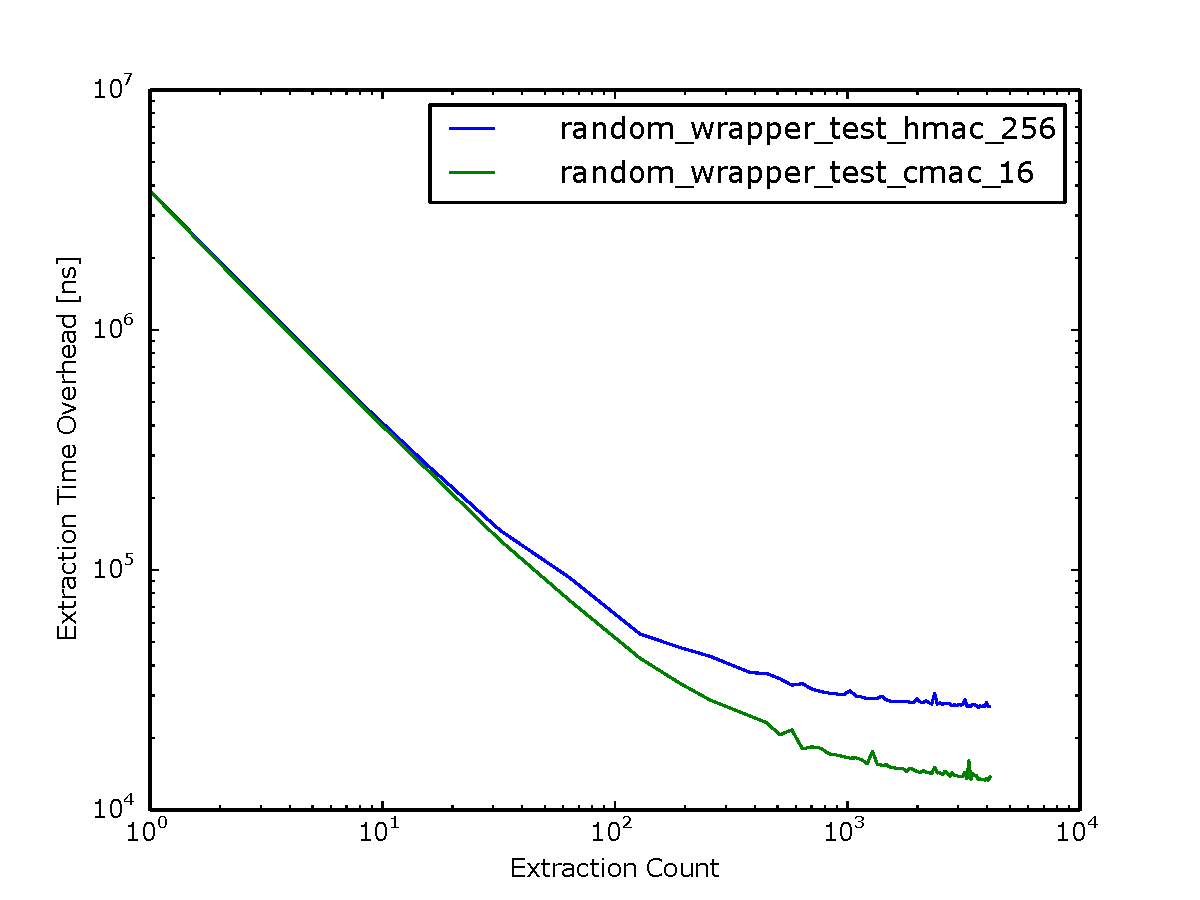
\includegraphics[width=\linewidth]{cost_1024.pdf}
		\caption{$B = 1024$}
		\label{fig:exp-d}
	\end{subfigure}
	\caption{Wrapper Experimental Overhead}
\end{figure}


\section{Version History}

\begin{itemize}
	\item[] v1.0 (2018-11-01) Original release
	\item[] v1.1 (2018-03-25) Major updates 
	\begin{itemize}
		\item Added Appendix A with wrapper experiments.
		\item Removed the redundant game (Game 1) from the proof.
		\item Clarified security properties of KDF (kdf security and uniformness preserving), modified the proof.
		\item Considered two cases of using HKDF-extract (direct and reverse orders of arguments).
		
	\end{itemize}
\end{itemize}
	
\end{appendix}

\end{document}
